\section{Comparing Models on Full Statistics Signal}

\subsection{Running on Full Statics}

\begin{figure}
    \makebox[\linewidth][c]{%
    \centering
    \begin{subfigure}{.85\textwidth}
        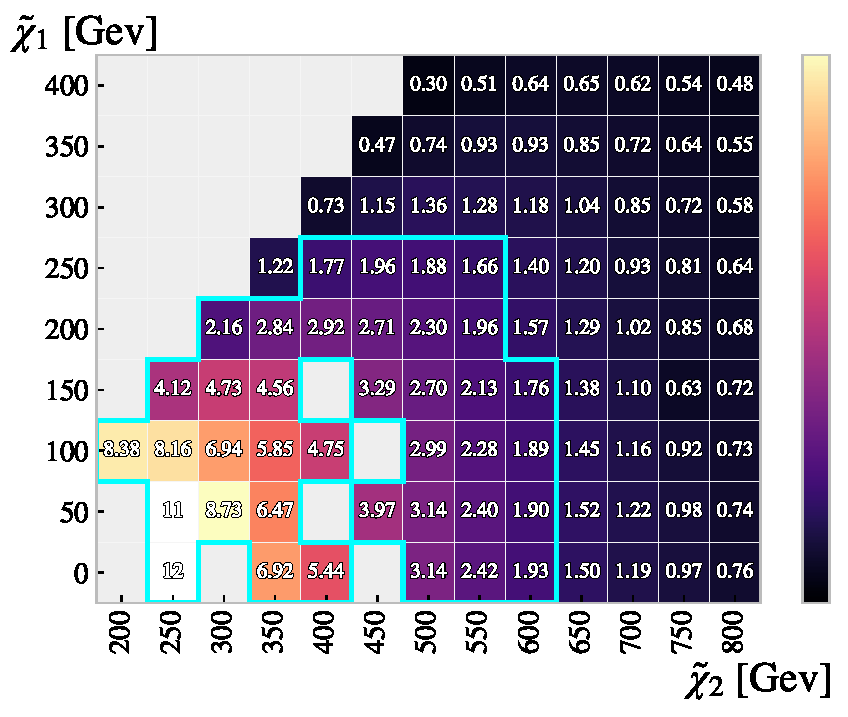
\includegraphics[width=\textwidth]{Figures/MLResults/NN/SUSY/Grid/FS/NN_FS_MLMGridSig.pdf}
    \end{subfigure}
    }
    \caption{A grid displaying the achieved significance on the full statistics signal set, using the signal region 
    created by the \emph{NN} network.}
    \label{fig:NN_FS_MLMGridSig}
\end{figure}

\begin{figure}
    \makebox[\linewidth][c]{%
    \centering
    \begin{subfigure}{.85\textwidth}
        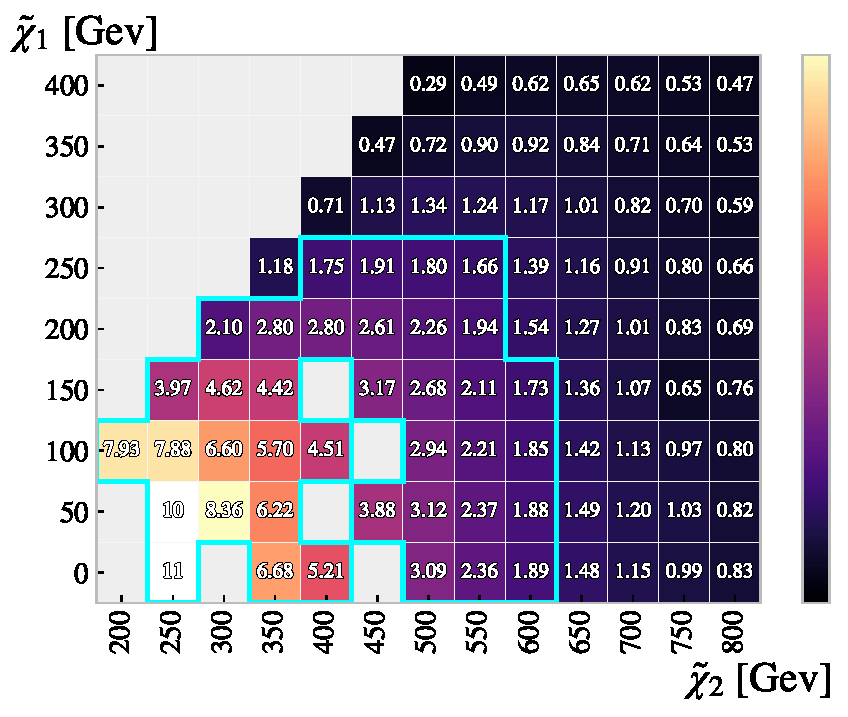
\includegraphics[width=\textwidth]{Figures/MLResults/NN/SUSY/Grid/FS/MaxOutPCA_FS_MLMGridSig.pdf}
    \end{subfigure}
    }
    \caption{A grid displaying the achieved significance on the full statistics signal set, using the signal region 
    created by the \emph{MaxOut} network.}
    \label{fig:MaxOutPCA_FS_MLMGridSig}
\end{figure}

\begin{figure}
    \makebox[\linewidth][c]{%
    \centering
    \begin{subfigure}{.85\textwidth}
        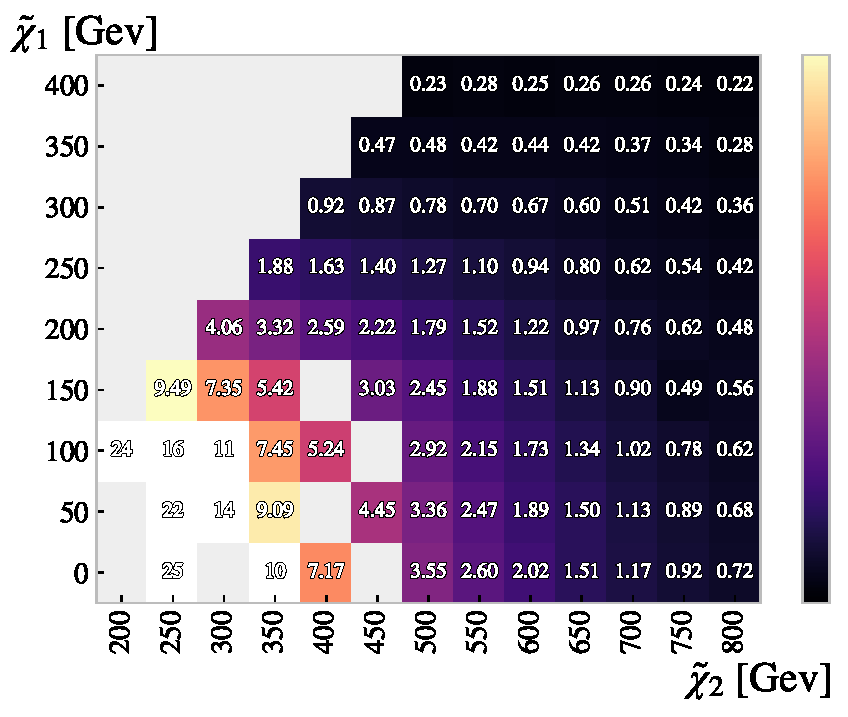
\includegraphics[width=\textwidth]{Figures/MLResults/NN/SUSY/Grid/FS/PNNPCA_FS_MLMGridSig.pdf}
    \end{subfigure}
    }
    \caption{A grid displaying the achieved significance on the full statistics signal set, using the signal region 
    created by the \emph{MaxOut} network.}
    \label{fig:PNNPCA_FS_MLMGridSig}
\end{figure}